\documentclass{beamer}
\usepackage{manfnt}
\usepackage{txfonts}
\usepackage{hyperref}
\usepackage{fancybox}
\usepackage{xfrac}
\usepackage{cancel}

\newcommand{\heart}{\ensuremath\heartsuit}

\usepackage{mathtools,amssymb}
\newcommand{\myarrow}{\scalebox{2}[2]{$\mathclap{\curvearrowleft}\mkern2.2mu
                                                 \mathclap{\curvearrowright}$}}

\DeclareMathOperator{\Bin}{\mathrm{Bin}}

\hypersetup{colorlinks=false,linkbordercolor=red,linkcolor=green,pdfborderstyle={/S/U/W 1}}

\addtobeamertemplate{navigation symbols}{}{ \hspace{1em}    \usebeamerfont{footline}%
    \insertframenumber / \inserttotalframenumber}

\geometry{papersize={15cm,13cm}}
\usepackage{lipsum}

\makeatletter
\newenvironment<>{contdproof}[1][\proofname]{%
    \par
    \def\insertproofname{#1\@addpunct{.}}%
    \usebeamertemplate{proof begin}#2}
  {\usebeamertemplate{proof end}}
\makeatother


\setbeamertemplate{theorems}[numbered]

\newtheorem*{nonumdefinition}{Definition}
\newtheorem*{nonumproblem}{Problem}
\newtheorem*{nonumtheorem}{Theorem}
\newtheorem*{nonumremark}{Remark}
\newtheorem*{answer}{Answer}
\newtheorem*{nonumremarks}{Remarks}
\newtheorem*{nonumexamples}{Examples}
\newtheorem*{nonumsolution}{Solution}
\newtheorem*{nonumexample}{Example}
\newtheorem*{nonumproposition}{Proposition}
\newtheorem{proposition}[theorem]{Proposition}

\usepackage{tikz}
\newcommand*\mycirc[1]{%
  \tikz[baseline=(C.base)]\node[draw,circle,inner sep=.7pt](C) {#1};\:
}

\newcommand\myheading[1]{%
  \par\bigskip
  {\color{blue}{\large #1}}\par\smallskip}

%\usetheme{Warsaw}
%\usetheme{Berkeley} %sample 1

\usetheme{Berlin} % sample 2
%\usetheme{AnnArbor} % sample 3

\let\otp\titlepage
\renewcommand{\titlepage}{\otp\addtocounter{framenumber}{-1}}

\title{Lecture 10 : Continuous Random Variables}
\author{}
\date{}

\begin{document}
\begin{frame}[plain]
\titlepage
\end{frame}

\begin{frame}
In this section you will compute probabilities by doing integrals.

\begin{nonumdefinition}
A random variable $X$ is said to be continuous if there exists a nonnegative function $f(x)$ definition interval $(-\infty,\infty)$ such that for any interval $[a,b]$ we have,
$$
P(a\leq X\leq b)=\int\limits^{b}_{a}f(x)dx
$$
\end{nonumdefinition}
\end{frame}

\begin{frame}
\begin{nonumdefinition}[Cont.]
$f(x)$ is said to be the probability density function of $X$, abbreviated pdf.

The usual geometric interpretation of the integral $\int^{h}_{a}f(\infty)dx$ as the area between $a$ and $b$ under the graph of $f$ will be very important later 

\medskip
\centerline{
\includegraphics{figure/fig1.eps}}
\smallskip

\end{nonumdefinition}
\end{frame}

\begin{frame}
\begin{itemize}
\item[\dbend] $f(x)\neq P(X=x)$ in fact $f(x)$ is not the probability of anything $f$ is a {\it density} i.e., something you integrate to get the magnitude of a physical quantity.
\end{itemize}

Think of a wire stretching from $a$ to $b$ with density $\lambda \dfrac{gm}{cm}$

\medskip
\centerline{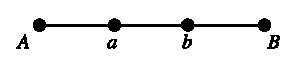
\includegraphics{figure/fig2.eps}}
\smallskip

Then the actually mass of the wire between $a$ and $b$ is $\int^{b}_{a}\lambda (x)dx$.
\end{frame}

\begin{frame}
So $\lambda$ is mass per unit
$$
\text{length}\qquad \lambda(x)=\lim \dfrac{\triangle m}{\triangle x}
$$
Similarly $f(x)=$ probability per unit length.

Both $\lambda$ and $f$ are derivatives of functions whose values have meaning.

\myheading{Properties of $f(x)$}

\begin{itemize}
\item[(i)] $f(x)\geq 0$ $\leftarrow$ no immediate physic interpretation, see later.

\item[(ii)] $\int^{\infty}_{-\infty}f(x)dx=1$ $\leftarrow$ total probability = 1
\end{itemize}
by function $f$ satisfying (i) and (ii) is a proof.
\end{frame}

\begin{frame}
\myheading{Example : The Uniform Distribution on $[0,1]$}

\myheading{Physical Problem}

Pick a random number in $[0,1]$ 

Call the result $X$.

So $X$ is a random variable.

\myheading{Questions}

What is $P\left(X=\dfrac{1}{2}\right)$?

What is $P\left(0\leq X\leq \dfrac{1}{2}\right)$

What is $P\left(\dfrac{1}{4}\leq X\leq \dfrac{3}{4}\right)$
\end{frame}

\begin{frame}
So we arrive at for $[a,b]$ inside $[0,1]$
$$
P(X\in [a,b])=P(a\leq X\leq b)=b-a =\text{ length } ([a,b])
$$
This is a continuous random variable. The density function is the ``characteristic function of $[0,1]$'' i.e.,
$$
f(x)=
\left\{
\begin{array}{ll}
1, & 0\leq x\leq 1\\
0, & \text{otherwise.}
\end{array}
\right.
$$

\centerline{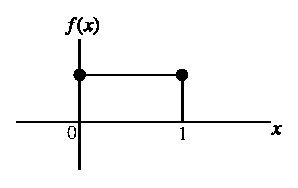
\includegraphics{figure/fig3.eps}}
\end{frame}

\begin{frame}
\begin{nonumdefinition}
A continuous random variable $X$ is said to have uniform distribution on $[0,1]$, abbreviate $X\sim \bigcup (0,1)$ if its pdf $f$ is given by
$$
f(x)=
\left\{
\begin{array}{ll}
1, & 0\leq x\leq 1\\[3pt]
0, & \text{otherwise.}
\end{array}
\right.
$$
More generally suppose we replace $[0,1]$ by the interval $[a,b]$
\begin{itemize}
\item[\dbend] We can't have
$$
f(x) = \cancel{
\left\{
\begin{array}{ll}
1, & a\leq x\leq b\\[3pt]
0, & \text{otherwise.}
\end{array}
\right.}
$$
\end{itemize}
\end{nonumdefinition}
\end{frame}

\begin{frame}
Why

\medskip
\centerline{
\includegraphics{figure/fig4.eps}}
\smallskip

So we have to define
$$
f(x)=
\left\{
\begin{array}{cl}
\frac{1}{b-a}, & a\leq x\leq b\\
0, & \text{otherwise}
\end{array}
\right.
$$
Then \ $\int^{b}_{a}f(x)dx=1$

\medskip
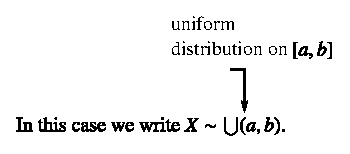
\includegraphics{figure/fig5.eps}
\end{frame}

\begin{frame}
\myheading{Another Example}

\myheading{Linear density}

\medskip
\centerline{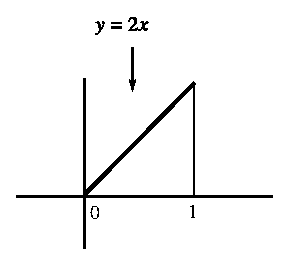
\includegraphics{figure/fig6.eps}}
\smallskip

Consider the function
$$
f(x)=
\left\{
\begin{array}{ll}
2x, & 0\leq x\leq 1\\
0, & \text{otherwise}
\end{array}
\right.
$$
Then the total probability is
$$
\int\limits^{\infty}_{-\infty}f(x)dx=\left.\int\limits^{1}_{0}2x=(x^{2})\right|^{x=1}_{x=0}=1
$$
\end{frame}

\begin{frame}
Since $f(x)\geq 0$ and
$$
\int\limits^{\infty}_{-\infty}f(x)dx=1~~ f(x)\quad\text{is}
$$
indeed a pdf.

\begin{nonumproblem}
For the linear density compute
$$
P\left(\dfrac{1}{4}\leq X\leq \frac{3}{4}\right)
$$
\end{nonumproblem}

\begin{nonumsolution}
\begin{align*}
P\left(\dfrac{1}{4}\leq X\leq \dfrac{3}{4}\right) &= \int\limits^{\infty}_{-\infty}f(x)dx=\int\limits^{\frac{3}{4}}_{\frac{1}{4}}2xdx\\[3pt]
&= (x^{2})\Big|^{x=\frac{3}{4}}_{x=\frac{1}{4}}=\frac{9}{16}-\frac{1}{16}=\frac{1}{2}
\end{align*}
No decimals please.
\end{nonumsolution}
\end{frame}

\begin{frame}
Here are some usual properties of {\it continuous} random variables.

They are all consequences of the fact that if $X$ is continuous and $c$ is any number then
$$
P(X=c)=0
$$

\begin{nonumtheorem}
\begin{itemize}
\item[(i)] $P(a\leq X\leq b)=P(a\leq X\leq b)$ (because $P(X=b)=0$)

\item[(ii)] $P(a\leq X\leq b)=P(a<X\leq b)$ (because $P(X=a)=0$)

\item[(iii)] $P(a\leq X\leq b)=P(a<X<b)$
\end{itemize}
{\it end points don't matter.}
\end{nonumtheorem}
\end{frame}

\begin{frame}
\myheading{Good Citizen Computations}

\myheading{The Cumulative Distribution Function}

\begin{nonumdefinition}
Let $X$ be a continuous random variable with pdf $f$. Then the cumulative distribution function $F$, abbreviate $cdf$, is defined by
$$
F(x)=\int\limits^{x}_{-\infty}f(x)dx
$$
= the area under the graph of $f$ to the left of $x$.
\end{nonumdefinition}
\end{frame}

\begin{frame}
\centerline{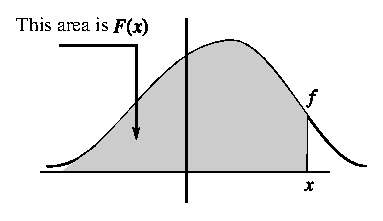
\includegraphics{figure/fig7.eps}}
\smallskip

We will compute the $cdfs$ for $X\sim \bigcup (0,1)$ and $X\sim$ the linear distribution.

\myheading{$X\sim \bigcup (0,1)$}

\centerline{
\includegraphics{figure/fig8.eps}}
\end{frame}

\begin{frame}
There will be {\it three} formulas corresponding to the {\it two} discontinuities in $f(x)$.

\myheading{$F(x)=0$, $x<0$}

This is clear because we haven't accumulated any probability/area get.

\medskip
\centerline{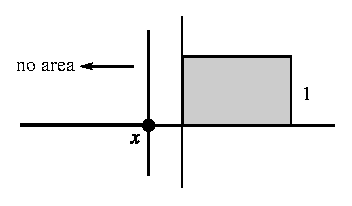
\includegraphics{figure/fig9.eps}}
\smallskip

\myheading{$F(x)=1$, $x>1$}

This is not quite so clean

\medskip
\centerline{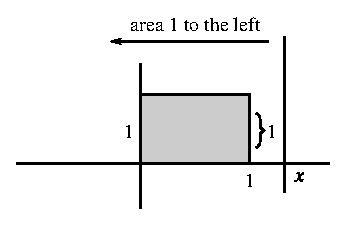
\includegraphics{figure/fig10.eps}}
\smallskip

We have over 1 to the left of $x$ and that's all we are going to set.
\end{frame}

\begin{frame}
\myheading{$F(x)=?$, $0\leq x\leq 1$}

This is where the action is.

\medskip
\centerline{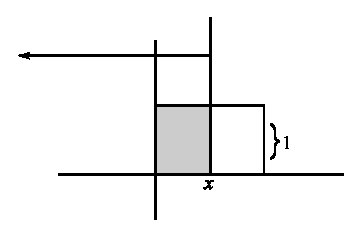
\includegraphics{figure/fig11.eps}}
\smallskip

How much area have we accumulated to the left of $x$. It is the area of a rectangle with base $x$ and height $1$ hence area $x-1=x$.

Thus \underline{$F(x)=x$, $0\leq x\leq 1$}

We could have done this with integrals instead of pictures but pictures are better.
\end{frame}

\begin{frame}
We have obtained
$$
F(x)=
\left\{
\begin{array}{ll}
0, & x<0\\
x, & 0\leq x\leq 1\\
1, & x>1
\end{array}
\right.
$$

\smallskip
\centerline{
\includegraphics{figure/fig12.eps}}
\smallskip

\myheading{Lesson}

$cdf$'s of continuous random variables are continuous and satisfy 
\begin{align*}
\lim\limits_{x\to -\infty}F(x)=0\\
\lim\limits_{x\to \infty}F(x)=1
\end{align*}
\end{frame}

\begin{frame}
\myheading{The $cdf$ of the linear distribution}

\medskip
\centerline{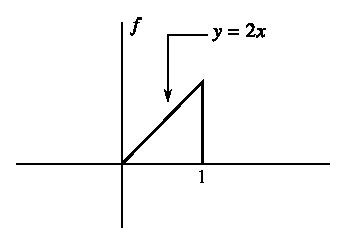
\includegraphics{figure/fig13.eps}}
\smallskip

We will go faster. Clearly again
\begin{align*}
& F(x)=0,\quad x<0\\[3pt]
\text{and}\qquad & F(x)=1,\quad x>1
\end{align*}
We have to compute $F(x)$ for $0\leq X\leq 1$.
\end{frame}

\begin{frame}
\centerline{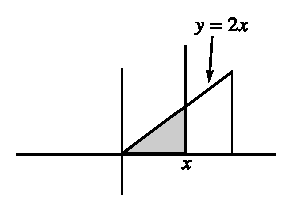
\includegraphics{figure/fig14.eps}}
\smallskip

\medskip
\centerline{\includegraphics{figure/fig15.eps}}
\smallskip

So we have to compute the area of a triangle with base $b=x$ and height $h=2x$. But
$$
\text{area~ } =\frac{1}{2} bh=\frac{1}{2}x(2x)=x^{2}
$$
So
$$
F(x)=
\left\{
\begin{array}{cl}
0, & x<0\\[3pt]
x^{2}, & 0\leq x\leq 1\\[3pt]
1, & x>1
\end{array}
\right.
$$
Do this with integrals.
\end{frame}

\begin{frame}
\myheading{Importance of the $cdf$}

Coded into the $cdf$ $F$ are all the probabilities $P(a\leq X\leq b)$.

\begin{nonumtheorem}
$P(a\leq X\leq b)=F(b)-F(c)$.
\end{nonumtheorem}

\begin{proof}
$P(a\leq X\leq b)=P(X\leq b)-P(X<a)$

But because $X$ is continuous
$$
P(X<a)=P(X\leq a)
$$
So
\begin{align*}
P(a\leq X\leq b) &= P(X\leq b)-P(X\leq 0)\\[3pt]
                 &= F(b)-F(a)
\end{align*}
\end{proof}
\end{frame}

\begin{frame}
\begin{nonumremark}
The previous theorem is critical. It is the basis of using tables (in a book or in a computer) to compute probabilities. A grid of values of $F$ (up to 10 decimal places say) are tabulated.
\end{nonumremark}

\begin{nonumtheorem}[How to recover the pdf from the $cdf$]
$F'(x)=f(x)$ at all points where $f(x)$ is continuous.
\end{nonumtheorem}
\end{frame}

\begin{frame}
\begin{nonumexample}
Suppose $X\sim \bigcup (0,1)$.

$F(x)$ has the graph

\medskip
\centerline{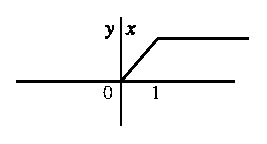
\includegraphics{figure/fig16.eps}}
\smallskip

So $F(x)$ is differential except at $0$ and $1$ and has derivative

\medskip
\centerline{\includegraphics{figure/fig17.eps}}
\smallskip

But this is $f(x)$. Note $f(x)$ is discontinuous of $0$ and $1$.
\end{nonumexample}
\end{frame}

\end{document}


